\section{Comparación global}

Esta sección resume la comparación final entre ambos enfoques, manteniendo foco en rendimiento en test, sensibilidad al umbral e implicaciones operativas.

\subsection{Desempeño predictivo en test}

Ambos modelos se evaluaron con el mismo protocolo (split externo 75/25 y validación cruzada estratificada 5-fold). La selección de umbral se realizó en validación interna y el contraste final en test.

\subsubsection{Métricas finales}

\begin{table}[h]
\centering
\small
\begin{tabular}{lccccccc}
\toprule
\textbf{Modelo} & \textbf{Umbral} & \textbf{Accuracy} & \textbf{Recall} & \textbf{Precisión} & \textbf{F1} & \textbf{ROC-AUC} & \textbf{PR-AUC} \\
\midrule
ET\_Recall  & 0.14 & 0.548 & 0.943 & 0.299 & 0.454 & 0.927 & 0.881 \\
RF\_Accuracy & 0.49 & 0.949 & 0.816 & 0.920 & 0.865 & 0.921 & 0.897 \\
\bottomrule
\end{tabular}
\caption{Desempeño final en el conjunto de test. ET: Extra Trees. RF: Random Forest.}
\label{tab:final_performance}
\end{table}

\begin{figure}[h]
\centering
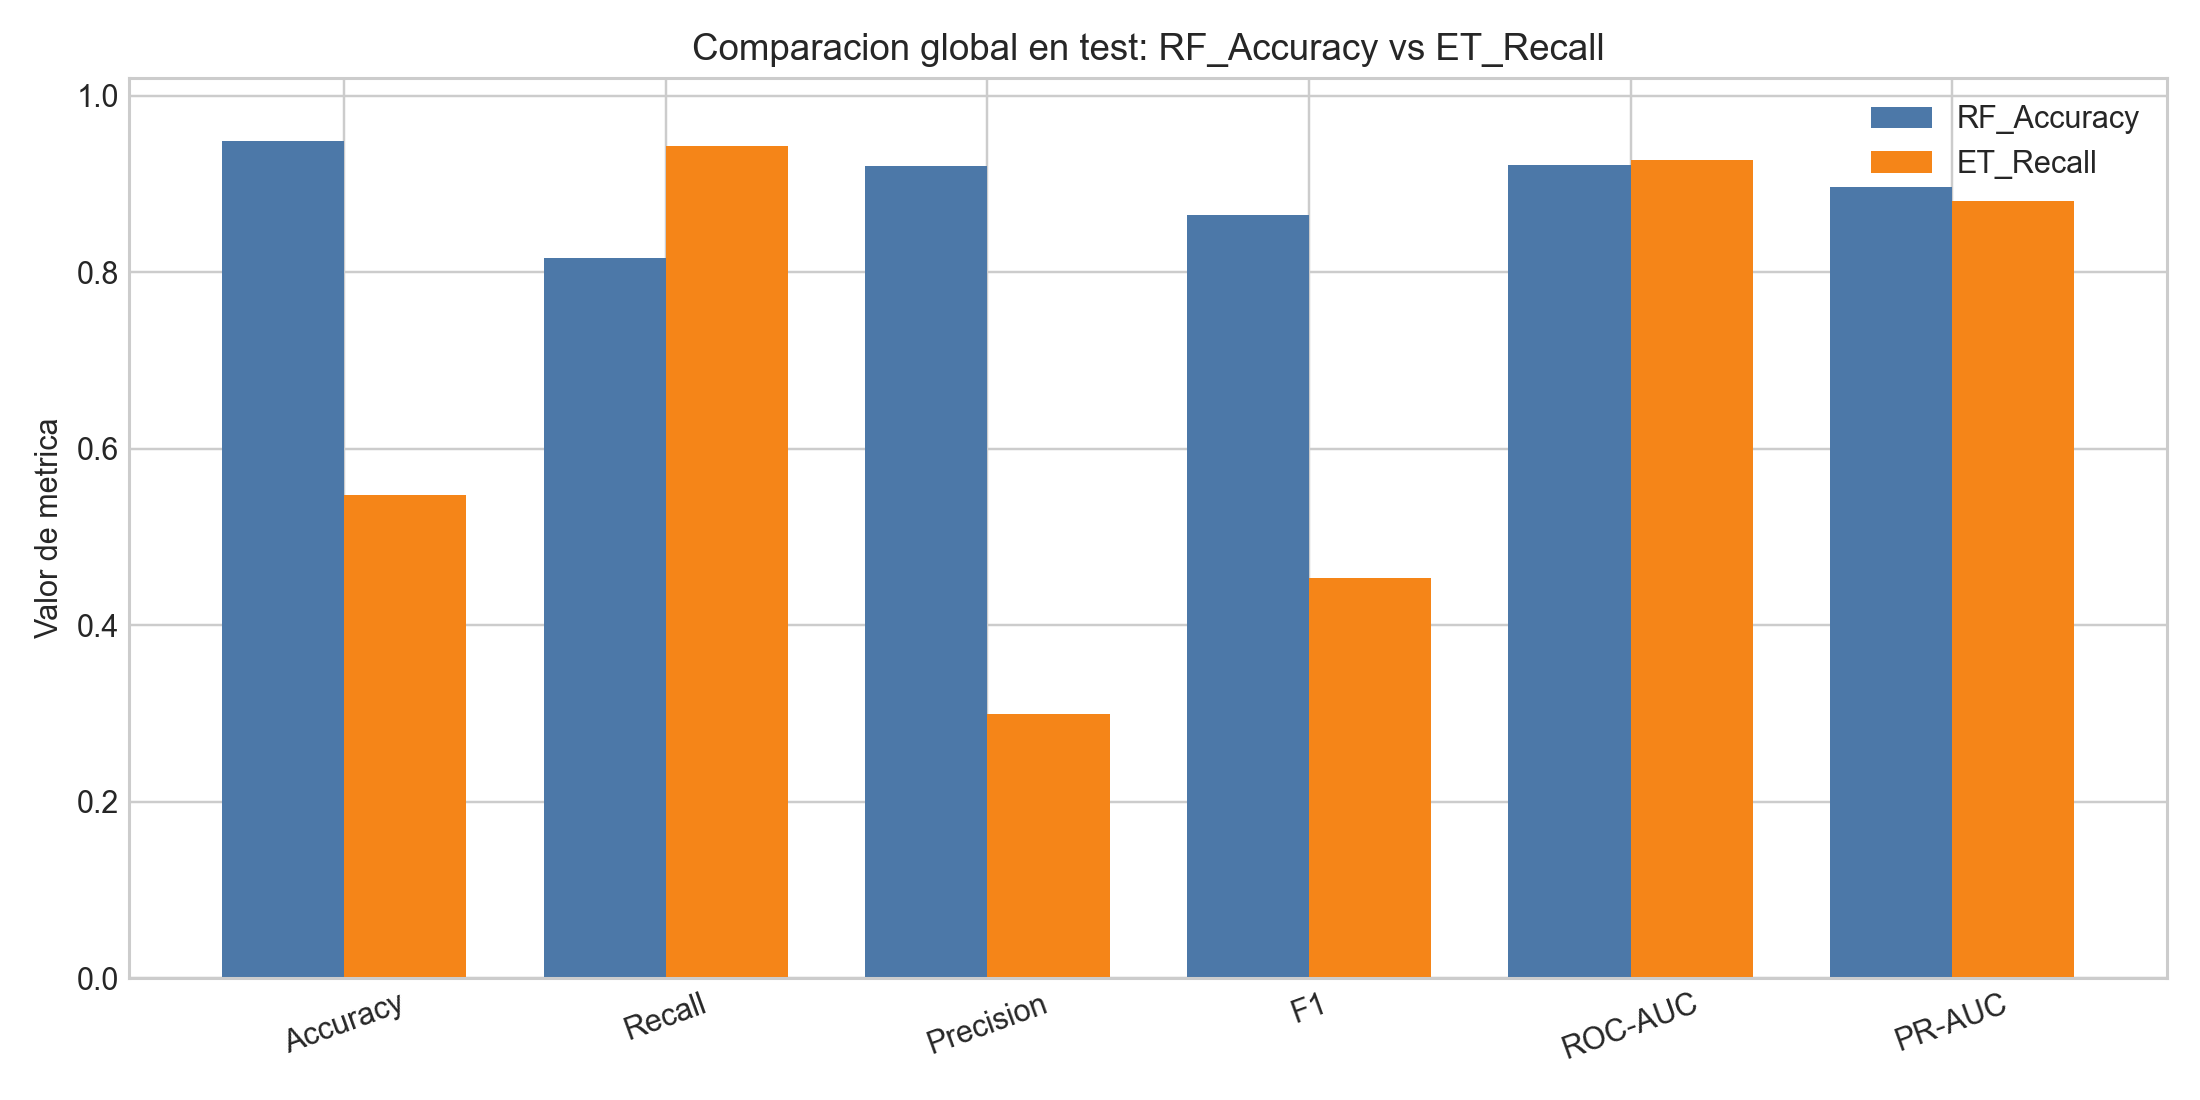
\includegraphics[width=0.92\textwidth]{figures/fase3_model_comparison_bars.png}
\caption{Comparación visual de métricas en test para RF\_Accuracy y ET\_Recall.}
\label{fig:comparacion_global_barras}
\end{figure}

RF\_Accuracy ofrece mejor desempeño global (Accuracy y Precision altas), mientras que ET\_Recall maximiza la cobertura de churn a costa de más falsos positivos.

\subsection{Trade-off entre objetivos}

El análisis del espacio de threshold confirma un intercambio claro entre cobertura y precisión:

\begin{itemize}
  \item \textbf{RF\_Accuracy}: su mejor compromiso se alcanza en threshold 0.49.
  \item \textbf{ET\_Recall}: mantiene recall alto con menor threshold, pero incrementa de forma notable los falsos positivos.
\end{itemize}

\begin{figure}[h]
\centering
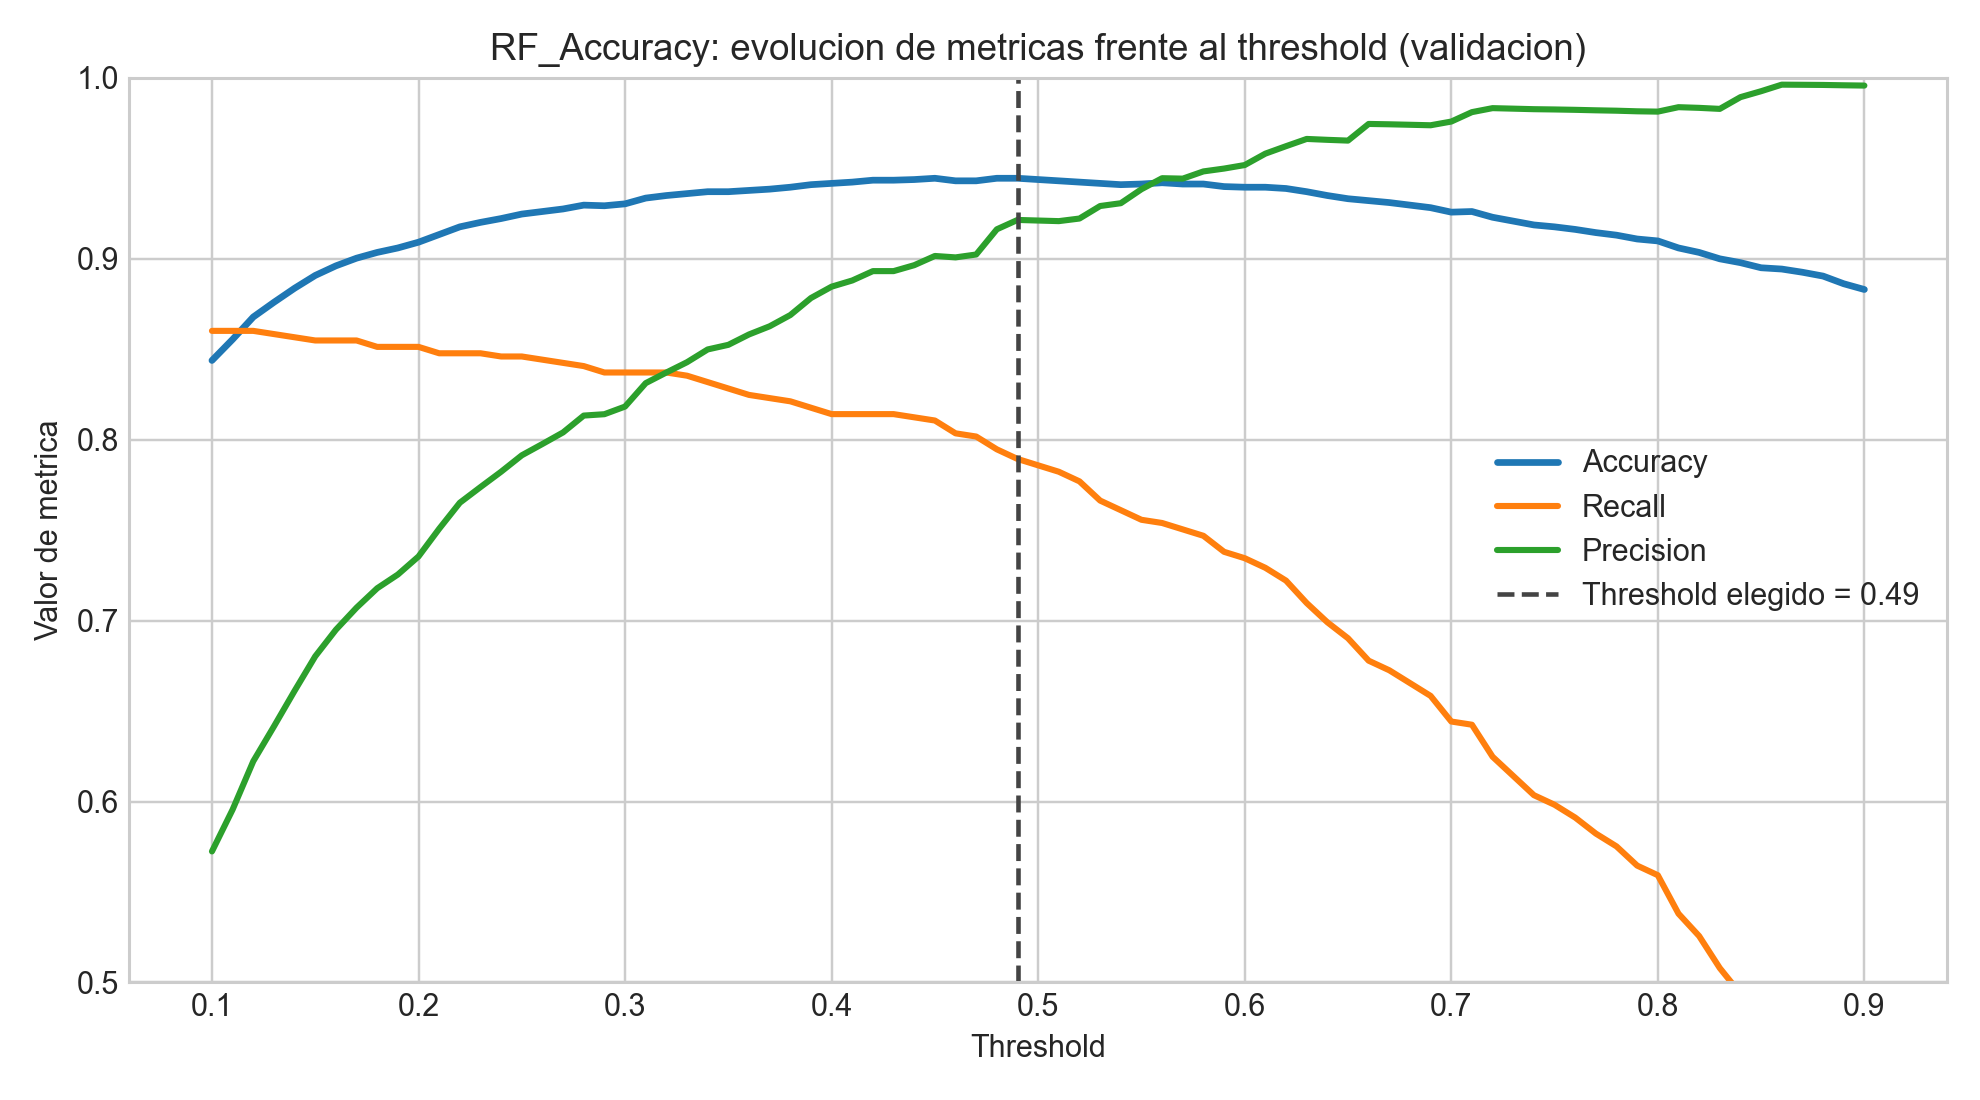
\includegraphics[width=0.9\textwidth]{figures/fase3_threshold_tradeoff_accuracy.png}
\caption{RF\_Accuracy: evolución de Accuracy, Recall y Precisión frente al threshold en validación.}
\label{fig:threshold_accuracy}
\end{figure}

\begin{figure}[h]
\centering
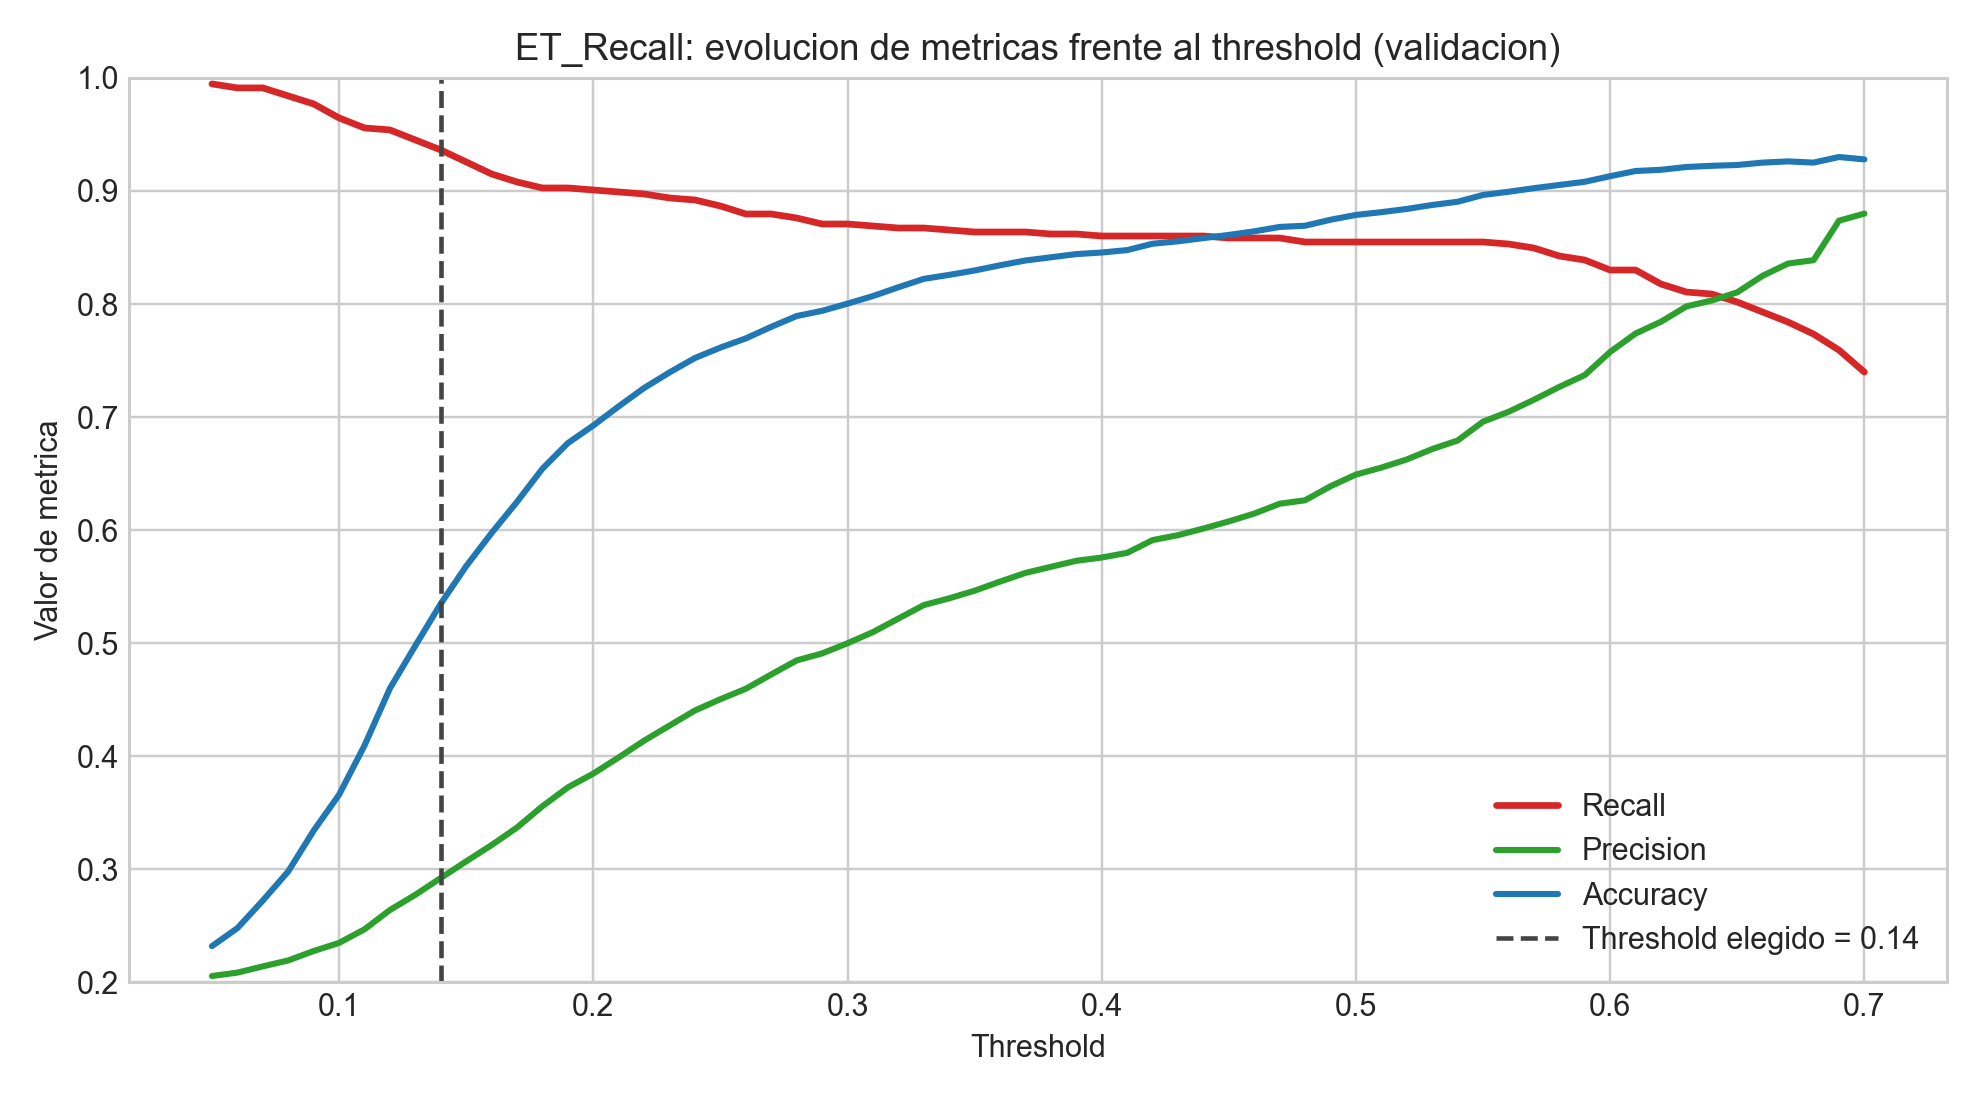
\includegraphics[width=0.9\textwidth]{figures/fase3_threshold_tradeoff_recall.png}
\caption{ET\_Recall: evolución de Recall, Precisión y Accuracy frente al threshold en validación.}
\label{fig:threshold_recall}
\end{figure}

\subsection{Sensibilidad de los guardrails para Recall}

El modelo ET\_Recall satisface los guardrails definidos:

\begin{itemize}
  \item \textbf{Precisión mínima:} 0.299 $>$ 0.25 \checkmark
  \item \textbf{PR-AUC mínimo:} 0.881 $>$ 0.80 \checkmark
\end{itemize}

Por tanto, ET es válido como modelo de alta cobertura, pero con mayor carga operativa.

\subsection{Síntesis operativa}

En términos de uso real, RF\_Accuracy es más eficiente cuando se prioriza precisión de campaña, mientras que ET\_Recall es útil como capa de exploración para no perder casos positivos.

\subsection{Recomendación}

Dado el contexto de retención de clientes:

\begin{enumerate}
  \item \textbf{Producción}: usar \textbf{RF\_Accuracy} como modelo principal por su mejor precisión global.
  \item \textbf{Análisis complementario}: usar \textbf{ET\_Recall} para ampliar cobertura y detectar casos potenciales no capturados por RF.
  \item \textbf{Monitoreo}: revisar periódicamente accuracy/recall para detectar deriva y ajustar threshold.
\end{enumerate}

En conclusión, \textbf{RF\_Accuracy} se selecciona como modelo principal y \textbf{ET\_Recall} se mantiene como apoyo para escenarios de cobertura máxima.
